\subsubsection{Thread Resistivity}
\begin{figure}
\centering
  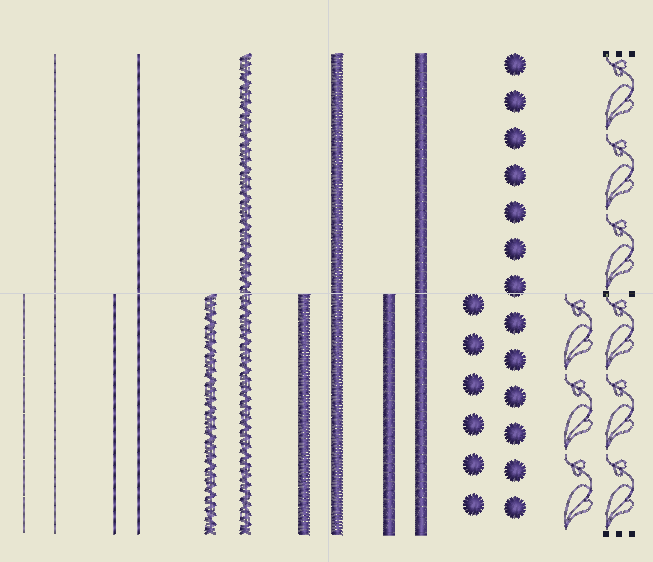
\includegraphics[width=0.9\columnwidth]{figures/Resistance}
  \caption{}~\label{fig:Resistance}
  \vspace{-2.5em}
\end{figure}
% the resistance of conductive thread is significant,
% which means that the placement of the electronic parts has
% to be taken into account when constructing circuits.



In our system, we us Consequently, for longer connections and power lines, the user can use, e.g., a satin stitch, to maintain low resistance. But while this technical solution serves its purpose, it might not be suitable for the design aesthetics.
 

\subsubsection{Electrical Insulation}
\begin{figure}
\centering
  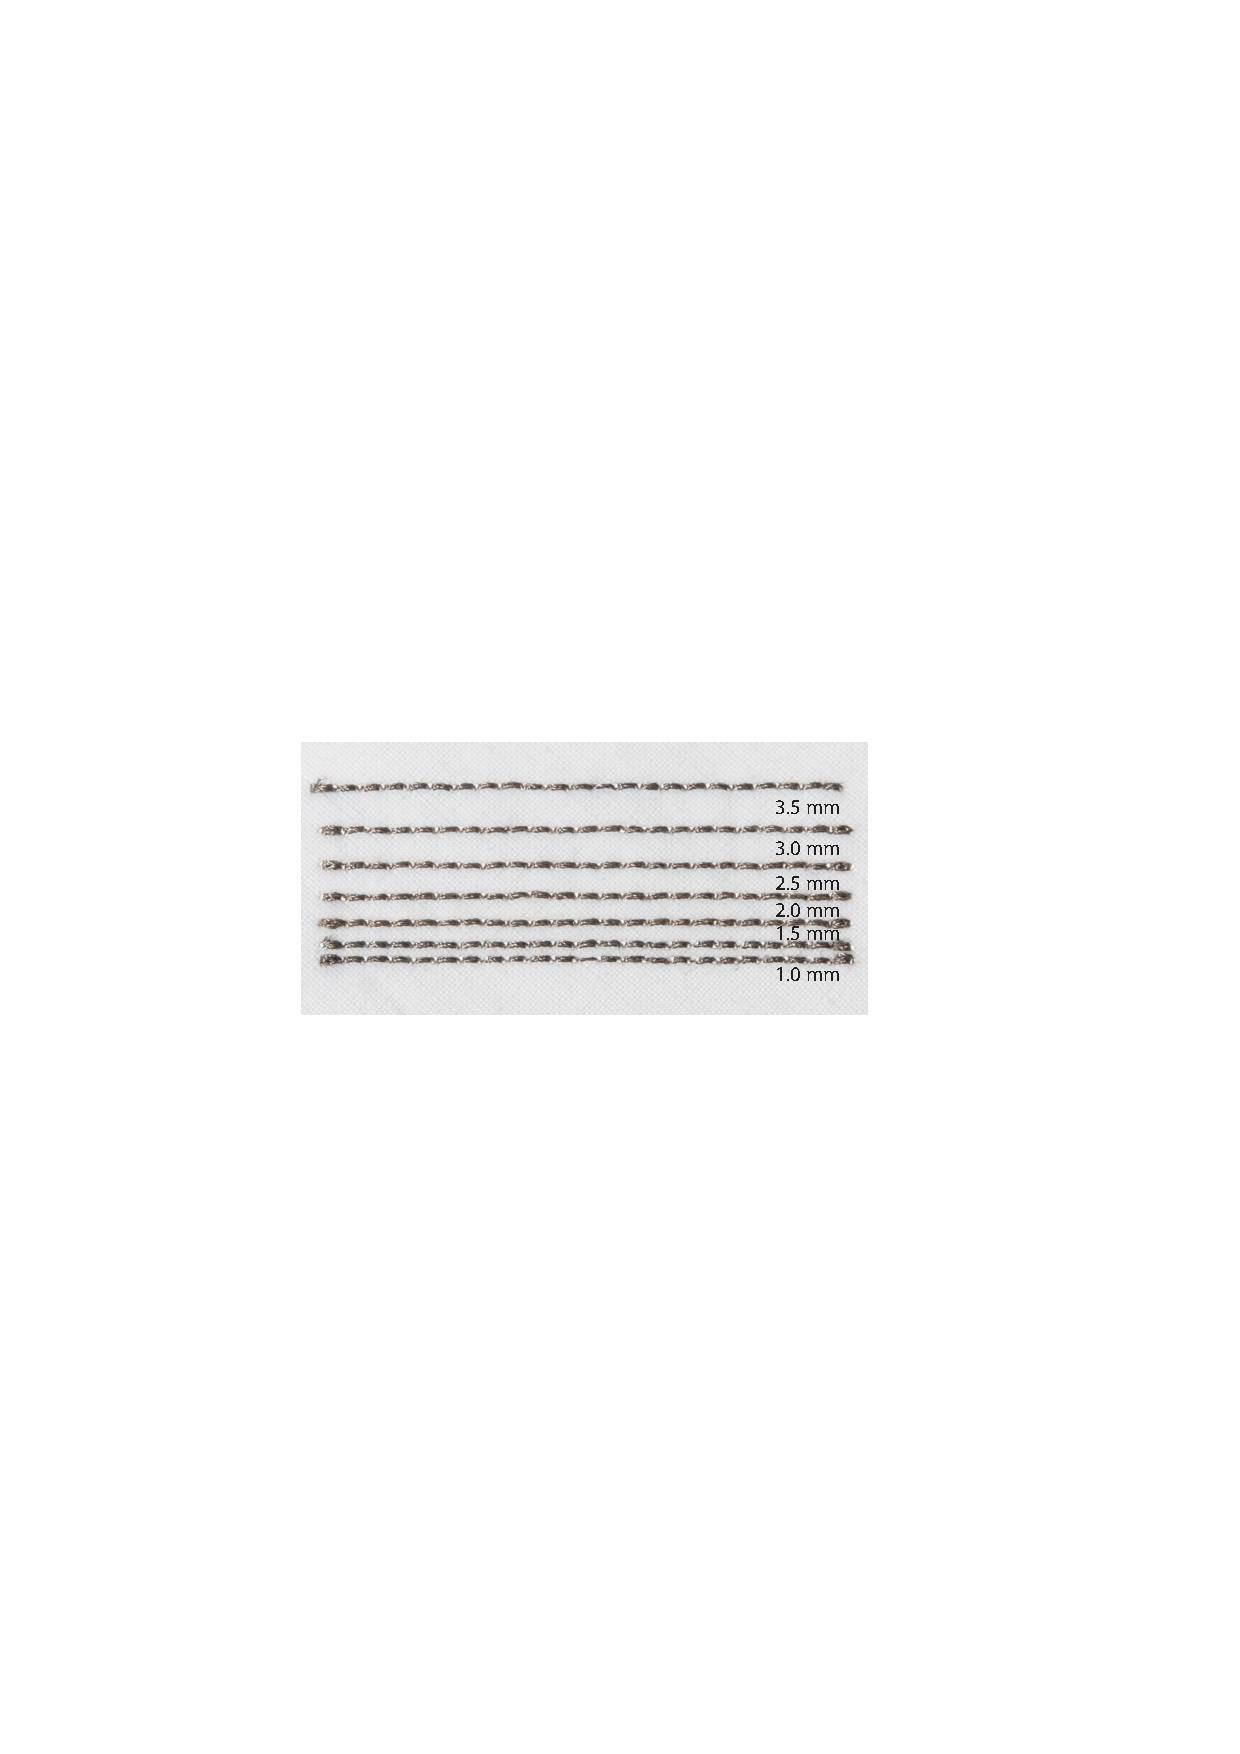
\includegraphics[width=0.9\columnwidth]{figures/Spacing}
  \caption{}~\label{fig:Spacing}
  \vspace{-2.5em}
\end{figure}
\begin{figure}
\centering
  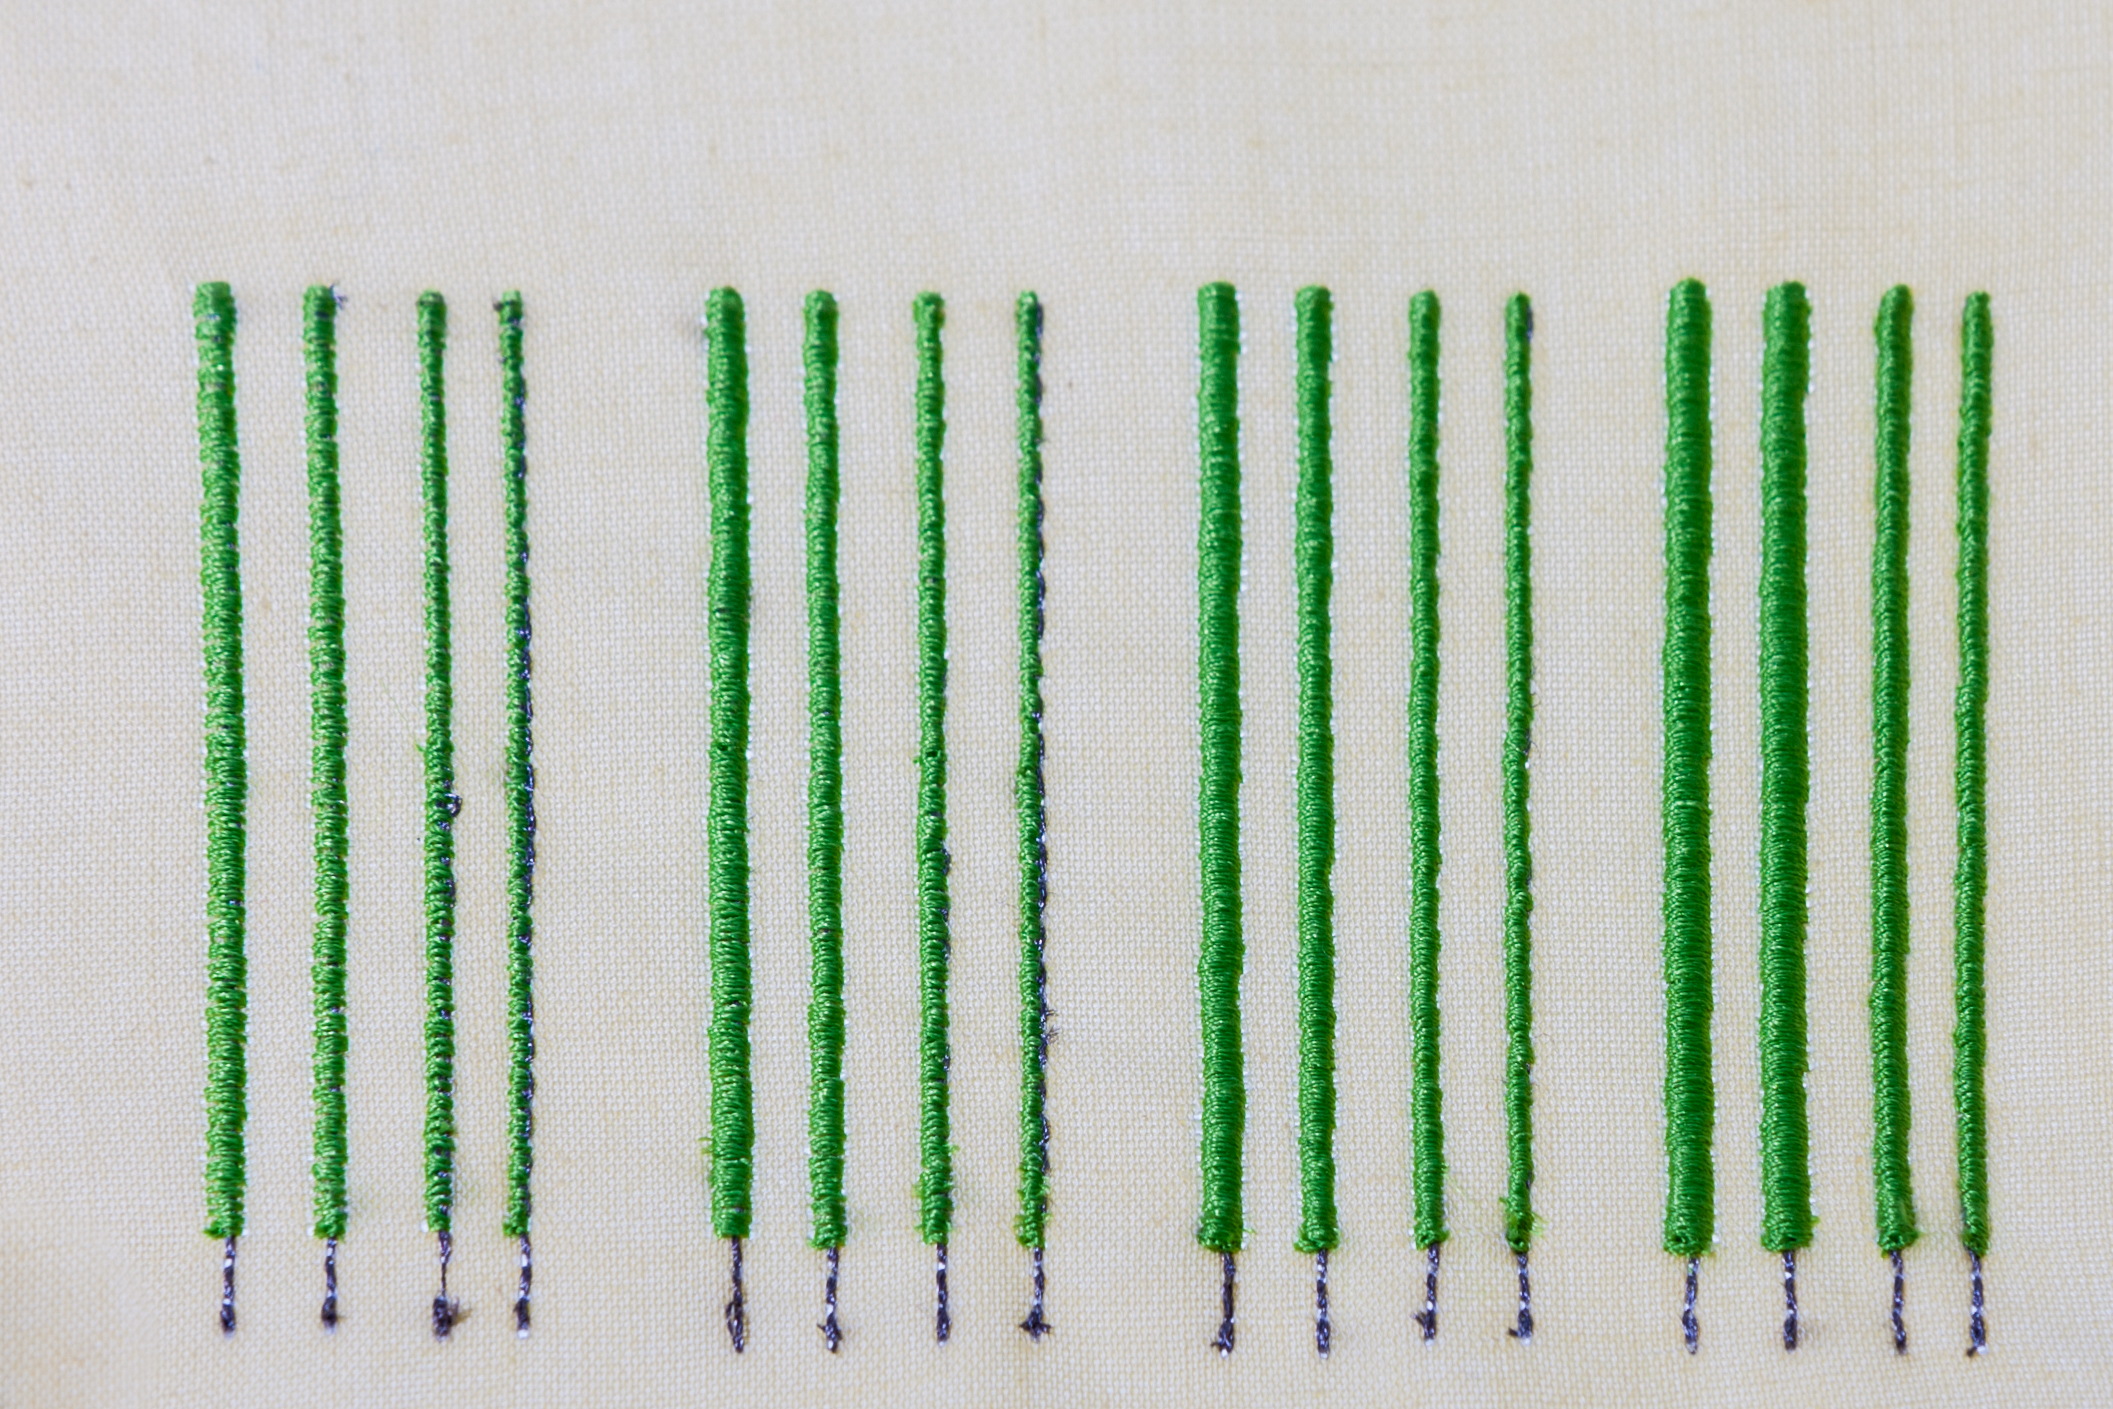
\includegraphics[width=0.9\columnwidth]{figures/Insulation}
  \caption{}~\label{fig:Insulation}
  \vspace{-2.5em}
\end{figure}
The composition and flexibility of conductive threads pose new challenges on users creating fabric circuits in comparison to wire-based circuits. Embroidery machine compatible conducive threads are made of short interlaced conductive fibers. As these fibers tend to be shorter than fibers in non-compatible threads, embroidery connection lines are more likely to fray \cite{5387040}. This can cause short circuits between adjacent lines. We address this challenge in two ways: a) increase the distance between any two lines to be more than 2.5 mm (this varies between threads based on the length of the composing fibers); and b) insulate the connections by covering them with non-conductive thread. Insulating the connections is also necessary for preventing undesired connections during fabric movement.

Previous work recommends insulating conductive
thread stitches with couching stitches or with puffy
fabric glue \cite{Buechley2009}. Our goal is to find a stitch pattern than can be atomically applied to electrical connections. We tested zigzag couching stitches with variable widths and stitch spacings. Figure X shows that the insulation stitch should be twice as wide as the underlying conductive thread to avoid side fraying. It also demonstrates that a zigzag stitch with spacing lower than 0.6mm in recommended to avoid accidental contact during movement.

\subsubsection{Overlap Stitch}
Tighter insulation with a loser run stitch.

\subsubsection{Rectangular Stitch: Embroidering Electrical Components}
We developed a stitch that can be used to embroider sewable electronics, e.g., LilyPad components, using the embroidery machine. Sewable electronics have holes, instead of pins, plated with a conductive material from the top and bottom sides of the PCB board. The holes are suitable for the needle size, e.g., LilyPad holes are 3 mm in diameter. We developed the \textit{rectangular stitch}, a top stitch pattern composed of four needle points arranged in a rectangular shape (see Figure). The needle moves between the four points several time to create a strong bond between the hardware and fabric. A connection line can be extended from the rectangular stitch to the fabric circuit.

The shorter sides of the rectangular stitch are 1.5 mm long, the long sides are 9 mm long. Two points of the rectangle are stitched inside the hole of the PCB (inner points), and two points are stitched 5 mm away from the PCB edge (outer points).  We modified a top stitch to have a minimum distance of 9 mm between subsequent needle points. This distance accounts for a) the distance between the center of pin hole and the edge of the PCB (\~ 4 mm), and b) the distance between the tip of the needle and the outer edge of the presser foot (\~5 mm). Reducing the stitch distance will lead the presser foot to push against the edge of the PCB when stitching close to it. On the other hand, increasing the distance can weaken the strength of the connection. A rectangular pattern was used, as opposed to a simple line, to distribute the number of repeated stitches between more needle points. Repeating a stitch in the same location creates a hole in the fabric at the needle point and may loosen the stitch. The rectangular stitch is limited to seawable electronics and requires precise alignment and stable fixation of electronics on fabric during embroidery.


%For context, the LilyPad kit uses an 0.8 mm PCB board for all its components. The presser-foot can successfully travel over the LilyPad PCB, but it hits the mounted SMDs (LEDs, resistors, speaker, microcontroller, etc.).


\subsection{Embroidery Sensors}
\subsubsection{Capacitive Sensors} 
\begin{figure}
\centering
  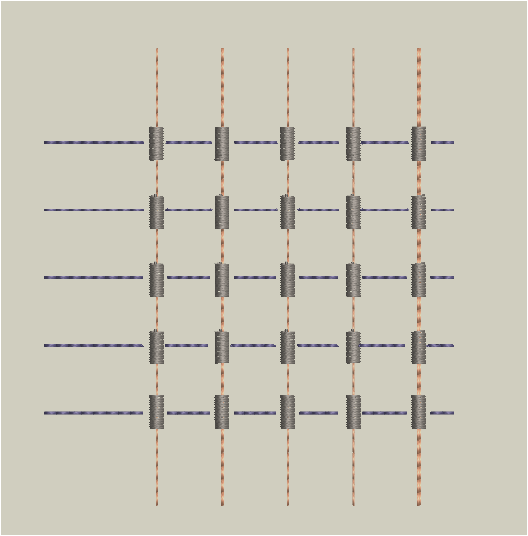
\includegraphics[width=0.9\columnwidth]{figures/MatrixCapacitor}
  \caption{}~\label{fig:MatrixCapacitor}
  \vspace{-2.5em}
\end{figure}

One can create a single capacitive touch point, e.g., a button, by filling an area on the fabric using conductive thread. This area can be of any shape or size. Fig x shows capacitive buttons with various Fill Stitches. All variations can be used to detect simple touch/no touch. Spars fills, such as ...., require less conductive thread (X - N stitches/cm\textsuperscript{2}) and provide a more textured surface. Dense fills, e.g., , can be used to create 2.5D visual and haptic effects but require more thread (C - V stitches/cm\textsuperscript{2})). To detect user touches, a capacitive touch area should be connected via a conducive thread connection to a microcontroller capable of capacitive sensing.

By repeating the touch points in a grid format, one can create a 2D capacitive touch area. We recommend that the spacing between any two touch points in the grid to have spacing larger than 2 mm to avoid permanent contacts and less than 10 mm to guarantee that a finger placed on the sensor will be detected by at least one touch point. One limitation of this technique is that each touch points needs to be connected to a dedicated pin on the microcontroller. In addition, when the number of touch points increases, the connection points will run closer to each other risking the chance of permanent connections. 

Alternatively, one can reduces the required number of pins and connections lines by creating a two layer grid layout. For example, a touch area of 16 points will require 4 horizontal connection lines interesting with 4 vertical connection lines to create 16 intersection points. At the intersection points an overlap stitch is applied between the overlapping lines preventing them from contacting each other. When the user touches an intersection point (Simon magic happens) and a touch is detected. This grid technique can be used as a Fill Stitch pattern to any shape.



\subsubsection{Resistive Sensors} 
\begin{figure}
\centering
  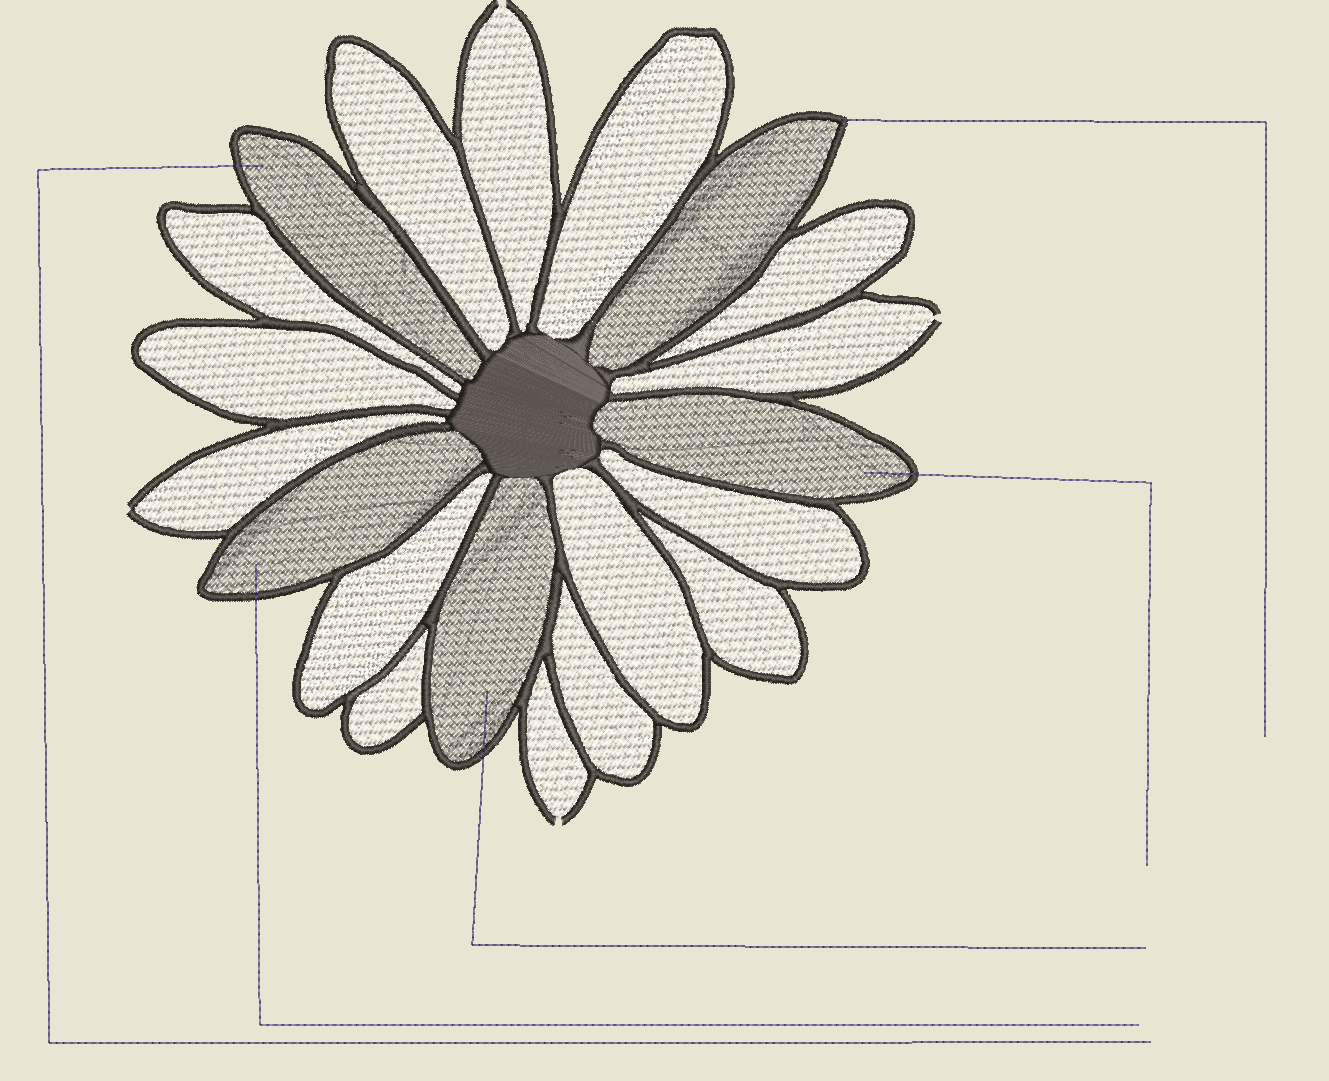
\includegraphics[width=0.9\columnwidth]{figures/FlowerSensor}
  \caption{}~\label{fig:FlowerSensor}
  \vspace{-2.5em}
\end{figure}
A resistive contact point requires two separate conductive areas, one connected to ground the other to a power source/data pin, that can be physically brought into contact, e.g., via pinching/folding them together []. A grid of contact points can be created. Using machine learning algorithm such as [], the location and orientation of the pinch can be detected and used for input.

\subsubsection{Pressure Sensor} 
Piezo resistive material (e.g., ) has similar chars as fabric and when sandwiched between a grid of conductive lines, it can be used to detect pressure level of a contact at the intersection points. This setup has been used by researchers, e.g., [], to study pressure sensitive textile sensors. However, since the conductive grid is created separately from the final construction, e.g., by cutting and gluing stripes of conductive fabric to form a grid, or purchasing woven pinstripe materials, connecting the sensor to a sensing controller is a challenge. Alternatively, we propose embroidering the grid lines, and extending them to a shred ``landing area'' on the same fabric. Figure X, demonstrates a X by Y grid. Piezo fabric is sandwiched between the two sides of the grid, and using the clipping mechanisms from [] we are able to attach a custom made PCB board on the landing area. This technique avoids the user of wires and creates a compact solution with reliable connections.  

We can also use the 2D capacitive grid method if we use piezo resistive thread in the overlap stitch instead of non-conductive thread.




%\section{E-Patches: Read-to-use textile components}
%Passive.
%Textile base for off-the-shelf electronics.

%Interactive Embroidery (IE) is a system that enables users to realize artistic e-textile artifacts quickly and easily. It allows users to work directly with the fabric rather than design software, simulating the traditional craft ways.
